\definecolor{darkgreen}{rgb}{0.0, 0.5, 0.0}
\lstdefinestyle{mystyle}{
    backgroundcolor=\color{white}, % pozadí kódu
    commentstyle=\color{green},
    keywordstyle=\color{blue},
    numberstyle=\tiny\color{gray},
    stringstyle=\color{darkgreen},
    basicstyle=\ttfamily\footnotesize,
    breakatwhitespace=false,
    breaklines=true,
    captionpos=b,
    keepspaces=true,
    numbers=left,
    numbersep=5pt,
    showspaces=false,
    showstringspaces=false,
    showtabs=false,
    tabsize=2,
    frame=single,
}
\lstset{style=mystyle}
% Změna textu "Listing" na "Ukázka"
\renewcommand\lstlistingname{Ukázka}
\renewcommand\lstlistlistingname{Ukázky kódu}

\section{Procedurální generování obsahu (PCG)}

Zpracováno na základě: \cite{PCGinG} \cite{HistoryOfPCG}.

Procedurální generování je metoda algoritmického vytváření dat. Procedurálně vytvořená data se od ručně vytvořených dat liší v tom, že jsou generována kombinací malého množství ručně vytvořených vstupních dat, na jejichž základě počítač podle daného algoritmu vytváří komplexnější výstup. Tento přístup je vhodný zejména pro aplikace, kde je vyžadováno velké množství různorodého obsahu nebo kde je ruční tvorba neefektivní.

Hlavní výhodou procedurálního generování je úspora času, lidských zdrojů a tím i finančních nákladů. Navíc umožňuje vytvořit obsah, který může být přizpůsoben konkrétním požadavkům nebo preferencím uživatele. Generovaný obsah je dynamický, což otevírá možnosti pro personalizaci zážitků, jako je například tvorba jedinečných map ve hrách nebo simulace náhodných prostředí.

\subsection{Výhody procedurálního generování}
Procedurální generování nabízí mnoho výhod, které ho činí atraktivním pro různé aplikace, hlavně ve vývoji her a designu:
\begin{itemize}
    \item \textbf{Redukce nároků na úložiště:} Namísto ukládání velkého množství dat je možné ukládat pouze algoritmus a jeho vstupní parametry.
    \item \textbf{Variabilita:} Algoritmus může generovat nekonečné množství unikátních výsledků.
    \item \textbf{Dynamika:} Obsah se může přizpůsobovat v reálném čase na základě uživatelských interakcí nebo jiných faktorů.
    \item \textbf{Úspora lidských zdrojů:} Omezuje potřebu ruční práce při tvorbě rozsáhlých prostředí.
\end{itemize}

\subsection{Nevýhody a výzvy procedurálního generování}
Ačkoliv má procedurální generování mnoho výhod, existují také určité nevýhody a výzvy:
\begin{itemize}
    \item \textbf{Kontrola kvality:} Výstup algoritmu nemusí vždy splňovat očekávání nebo být konzistentní s požadovanými normami.
    \item \textbf{Složitost implementace:} Návrh a ladění algoritmů mohou být časově náročné.
    \item \textbf{Předvídatelnost:} Přílišná náhodnost může vést k obsahu, který nedává smysl nebo není použitelný.
    \item \textbf{Závislost na vstupních datech:} Kvalita výstupu je silně ovlivněna kvalitou a rozmanitostí vstupních dat.
\end{itemize}

\subsection{Procedurální generování ve hrách}

Kapitola zpracována s~pomocí: \cite{PCGinG} \cite{HistoryOfPCG}.

Procedurální generování obsahu hraje klíčovou roli v moderním herním vývoji, zejména díky schopnosti efektivně vytvářet rozsáhlé a rozmanité herní světy. Tento přístup je oblíbený především pro hry s otevřeným světem, jako jsou \emph{Minecraft}, \emph{No Man's Sky} nebo série \emph{Rogue-like} her, kde je kladen důraz na variabilitu a dynamické prostředí.

Procedurální generování umožňuje vytvořit herní světy, které jsou pro hráče vždy jedinečné, což zvyšuje atraktivitu a prodlužuje životnost hry. Například v \emph{Minecraftu} se každý nový svět skládá z unikátní kombinace biomů, terénních útvarů a zdrojů, což hráče motivuje k dalšímu průzkumu. Podobně ve hře \emph{No Man's Sky} je generováno celé univerzum s miliardami planet, z nichž každá má unikátní prostředí, faunu a flóru.

Hlavní výhodou využití PCG v herním designu je schopnost generovat obsah přizpůsobený hráčově zkušenosti. Například v akčních hrách mohou algoritmy procedurálního generování upravovat obtížnost úrovní v reálném čase na základě výkonu hráče. Tento adaptivní přístup může zajistit, že hra zůstane náročná, ale zároveň nefrustrující, což zvyšuje angažovanost hráče.

Dalším využitím PCG je tvorba náhodných misí nebo úkolů. Ty mohou být generovány tak, aby obsahovaly různé cíle, nepřátele nebo interaktivní objekty. Tento přístup umožňuje vytvořit dynamický herní zážitek, kdy žádná mise nebo průběh hry nejsou zcela stejné. Tento princip se často využívá například ve hrách typu \emph{Diablo} nebo \emph{Borderlands}, kde jsou zbraně a další vybavení generovány procedurálně.

I přes četné výhody s sebou procedurální generování přináší i určité výzvy. Například ve hře \textit{No Man's Sky} čelili vývojáři kritice za přílišnou repetitivnost obsahu, přestože byl generován procedurálně. Dalším problémem je zajištění smysluplnosti a konzistence herního světa, což vyžaduje pečlivě navržené algoritmy a pravidla.

\subsubsection{Procedurální generování textur a zvuků}
Procedurální generování nachází své uplatnění také při tvorbě textur a zvuků, což významně přispívá k redukci nároků na úložný prostor. Textury povrchů, jako jsou dřevo, kámen nebo kov, mohou být generovány pomocí algoritmů, jako je \textbf{Perlin Noise} nebo \textbf{Simplex Noise}. Také je tímto přístupem generovat vegetaci, tak aby každý strom a keř vypadal unikátně například pomocí \textbf{Grammar Algorithms}. Tento přístup nejen šetří místo na disku, ale také zvyšuje variabilitu, protože každá textura může být jedinečná.

Podobně lze procedurálně generovat zvuky, jako je ambientní hudba nebo efekty prostředí (například šum deště, větru či zvuky zvířat). Použitím technik syntézy zvuku místo ukládání statických zvukových souborů je možné dynamicky přizpůsobit zvukové efekty aktuálním podmínkám ve hře, čímž se nejen šetří úložiště, ale také zlepšuje ponoření hráče do herního prostředí.

Tento přístup umožňuje nejen vytváření efektivnějších her z hlediska úložných nároků, ale také otevírá dveře k větší míře personalizace a přizpůsobení herního obsahu konkrétním hráčům.




\section{Metody procedurálního generování map}

V rámci této práce využijeme procedurální generování specificky pro vytvoření nové herní plochy pro každou hru. V této části se podíváme na některé možné techniky pro generování herních map. Hlavními požadavky na algoritmy je logické rozložení map, hratelnost a rychlost generování.

Algoritmy byly mimo jiné zpracovány na základě: \cite{PCGinG}.

\subsection{Space Partitioning}

%Nepoužitý odkaz: https://gameprogrammingpatterns.com/spatial-partition.html

Dělení prostoru je metoda, která rekurzivně rozděluje herní mapu na menší, disjunktní oblasti, přičemž každý bod mapy náleží právě jedné z těchto oblastí. Výsledkem je hierarchická struktura, obvykle reprezentovaná stromem, která umožňuje rychlé vyhledávání informací a manipulaci s daty.

Hlavním principem této metody je postupné dělení základního prostoru, dokud nejsou splněny předem stanovené podmínky, jako je například minimální velikost buňky nebo místnosti. Tento přístup nachází uplatnění nejen při generování herních map, ale také v grafických aplikacích, jako je ray-tracing, kde umožňuje efektivně organizovat a vykreslovat objekty ve scéně. \cite{PCGclanek}.

Nejběžnější metoda pro rozdělování prostoru je \textit{binární dělení prostoru (BSP)}. Jde o proces, který opakovaně rozděluje prostor na dvě části, dokud nejsou splněny určité požadavky. Ukázka \textit{BSP} je zobrazena na obrázku \ref{BSP_ukazka}. Další často využívanou variantou je \textit{quadtree}, kde je prostor rozdělen na čtyři symetrické části. Hlavním rozdílem mezi \textit{quadtree} a \textit{BSP} je, že v \textit{BSP} nemusí být na rozdíl od \textit{quadtree} všechny buňky symetrické a buňky v \textit{BSP} navíc nemusí mít stejnou orientaci \cite{BSPclanek}.

Metoda je běžně využíváno při vykreslování grafických scén, kde se dělící roviny vybírají na základě polygonů, aby optimalizovaly výpočty. Pro renderování scény je například důležité zajistit, že každý uzel stromu obsahuje polygony, které lze vykreslit efektivně. \cite{BSPclanek}.

Princip dělení prostoru na disjunktní oblasti je také ideální pro vytváření místností nebo oddělených oblastí v herním levelu. Celý level je reprezentován jako kořen \textit{BSP}, jehož prostor je dělen, dokud nejsou splněny stanovené podmínky (například minimální velikost místností). \textit{BSP} zajišťuje, že se oblasti nebudou překrývat \cite{PCGclanek}.

\begin{figure}
  \centering      % vycentrovat
  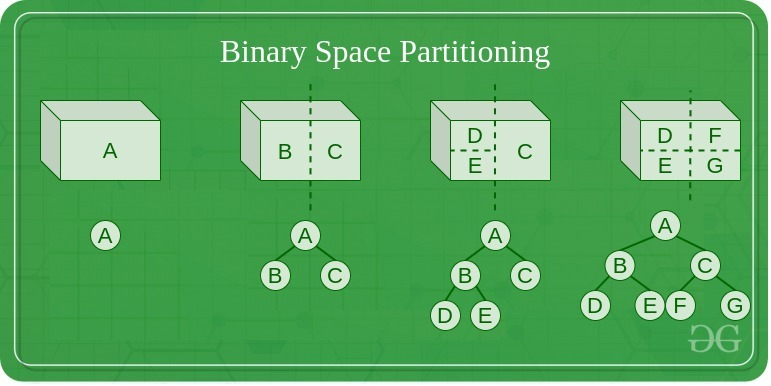
\includegraphics[scale=0.6]{obr/BSP.jpg} % soubor + měřítko (scale)
  \caption{Ukázka \textit{BSP} \cite{BSPclanek}} % popis obrázku
  \label{BSP_ukazka} % definice odkazu na obrázek (pro \ref{})
\end{figure}

\subsection{Agent-Based generování}
%Měl bych citovat každý odstavec když jsou všechny ze stejného zdroje?

Nejjednodušší \textit{agent-based} metoda přistupuje ke generování úrovní tak, že vygeneruje agenta který "vykopává" chodby a vytváří oblasti v souvislé sekvenci. Na rozdíl od přístupu dělení prostoru se jedná spíše o mikro přístup ke generování to vede k organicky vypadajícím výsledkům, které však mohou být chaotické a může docházet k překrývání místností. 

Těmto problémům se dá do nějaké míry zabránit optimálním nastavením pravidel agenta, ale to je náročné a efekt změny parametrů je obtížné odhadnout bez testování.

Pro jednoduché generování úrovní existují dva hlavní přístupy: \textit{"slepého" agenta} a \textit{agenta s "přehledem" ("look-ahead")}

\subsubsection{Slepý agent}
Metoda se slepým agentem je stochastická a funguje tak, že: Agent začíná v náhodném bodě dungeonu, a náhodně se vybere směr (nahoru, dolů, vlevo nebo vpravo). Agent začne "kopat" tímto směrem, a každý vykopaný dlaždicový bod dungeonu je nahrazen "chodníkovou" dlaždicí. Po prvním "vykopání" je 5\% šance, že agent změní směr (vybere nový náhodný směr) a další 5\% šance, že agent umístí místnost náhodné velikosti. Každým dalším dlaždicovým bodem ve směru, který se shoduje s předchozím, se šance na změnu směru zvyšuje o 5\%. Každým dalším dlaždicovým bodem bez přidání místnosti se šance na přidání místnosti zvyšuje o 5\%. Když agent změní směr, šance na změnu směru se sníží na 0\%. Když agent přidá místnost, šance na přidání místnosti zůstává na 0\%.

\subsubsection{Agent s přehledem}
Metoda s agentem s přehledem řeší problémy slepé metody jako jsou překrývající místnosti a slepé chodby tím, že agenta informuje o vzhledu úrovně, tedy agent může kontrolovat co se stane když přidá místnost, zda dojde k propojení místností. Zároveň také agent díky přehledu může zvolit směr tak aby se dostal do oblasti kde nehrozí překrytí a tedy nehrozí, že všechny místnosti úrovně budou naskládané na sobě. \cite{PCGclanek}
%----
\subsubsection{Vícefázové generování terénu}
V kontrastu s těmito přístupy, existuje další metoda, která využívá agentů k vytváření složitějších terénů, a to prostřednictvím více fázového procesu.

Tento přístup využívá tři hlavní fáze generování terénu:

\begin{enumerate}
    \item Fáze pobřeží: V této fázi velké množství agentů pracuje na vytvoření obrysu pevninské masy, která může být obklopena vodou.
    \item Fáze terénu: V této fázi agenti definují vlastnosti mapy, jako je tvarování hor, nížin a pláží.
    \item Fáze eroze: V této fázi agenti vytvářejí řeky, které erodují terén a spojují horské oblasti s oceánem.
\end{enumerate}

Každý agent v tomto systému je schopen vidět aktuální výšku jakéhokoli bodu na mapě a může tyto body modifikovat podle potřeby. Tímto způsobem agenti aktivně formují terén a přítomnost jiných agentů může způsobit změny v okolním prostředí. Pro ovládání životnosti agenta je každý agent vybaven určitým počtem tokenů, které spotřebovává při vykonávání akcí. Tento mechanismus dává designérovi možnost ovlivnit, jak bude terén generován.

Designér může ovlivnit makro-vlastnosti mapy tím, že určí počet agentů v každé fázi a počet tokenů, které budou agenti mít k dispozici. To umožňuje vytvářet různé typy terénů, jako jsou například pobřežní oblasti, hory nebo řeky.

Tento přístup, využívající několik fází a různých typů agentů (pobřežní agenti, agenti hor, agenti řek, atd.), dává designérovi větší kontrolu nad výsledným terénem, což může vést k zajímavějším a strukturovanějším mapám než u jednodušších metod založených na jednom agentovi. \cite{Agent-basedClanek}


\subsection{Grammar Algorithms}

\textit{Gramatiky} jsou obecně způsob, jak popsat strukturu a rozebrat její pod části. Například věta může obsahovat podmět a ten může obsahovat přídavná jména. \textit{Gramatiky} lze ale také aplikovat mimo mluvené jazyky. Jednoduchým příkladem je binární strom, který může být strukturován následovně \ref{gramStrom1}. \cite{GramFand} \cite{GramClanek}
\begin{lstlisting}[language=php, caption=Příklad gramatiky: Strom, label=gramStrom1]
    BRANCH ->
        node BRANCH BRANCH |
        leaf
\end{lstlisting}
Tento typ algoritmu však nemůžeme generovat nové struktury. Pro generování nového obsahu můžeme takový algoritmus upravit přidáním nějakých pravděpodobností. Algoritmus pak s určitou pravděpodobností generuje jednotlivé části struktury – například věty nebo jiné objekty. Můžeme naznačit na ukázce stromu, váhy nastavíme tak, že je dvakrát vyšší pravděpodobnost vygenerování listu než rozdělení uzlu \ref{gramStrom2}. \cite{GramClanek}
\begin{lstlisting}[language=php, caption=Příklad gramatiky: Strom s váhami, label=gramStrom2]
    BRANCH ->
        node BRANCH BRANCH [weight=1] |
        leaf [weight=2]
\end{lstlisting}

Gramatiky jsou silným nástrojem pro generování herního obsahu, protože poskytují strukturovaný způsob, jak popsat a vytvářet různé herní prvky, od prostorových uspořádání po specifické herní objekty. Tento přístup je podobný tomu, jak generativní gramatiky popisují strukturu přirozených jazyků. Jak bylo uvedeno dříve, generativní gramatiky používají konečnou sadu rekurzivních pravidel k definování větších struktur z menších částí, což se ukazuje jako efektivní způsob generování komplexních herních prostorů.

Například je možné použít grafovou gramatiky pro generování topologie úrovní, kde uzly reprezentují místnosti a hrany mezi nimi určují jejich propojení. Tento přístup je velmi flexibilní, protože umožňuje přizpůsobit generování úrovní specifickým parametrům, jako je obtížnost, velikost nebo zábavnost. Tento vysoký stupeň kontroly je výhodný v kontextu her, kde je potřeba mít pod kontrolou herní zážitek, ale na druhou stranu může být složité vytvořit univerzální gramatiku, která by pokryla všechny možné herní scénáře.

Když se vrátíme k použití pravděpodobnostních gramatik, jako ukázáno v předchozím příkladu s binárním stromem, přidání váhových faktorů umožňuje algoritmu vytvářet výsledky s různou pravděpodobností. Tato metoda může být efektivně aplikována na generování úrovní, kde například existují různé pravděpodobnosti pro výskyt místností určité velikosti nebo pro přítomnost specifických herních objektů. Tímto způsobem lze vytvářet náhodné, ale zároveň logické a konzistentní herní prostory, které odpovídají požadavkům designu. \cite{PCGclanek}



\subsection{Výškové mapy}

Terén může být snadno reprezentován jako dvourozměrná matice reálných čísel, kdy šířka a výška matice odpovídají rozměrům \textit{x} a \textit{y} a hodnoty v jednotlivých buňkách představují výšku v daném bodě. Takové matici se říká \textit{výšková mapa (heightmap)}. \cite{NoiseClanek}

\subsubsection{Náhodný terén}

Nejjednodušší metodou jak výškovou mapu vytvořit, je použít generátor náhodných čísel a matici jednoduše vyplnit náhodnými čísly. Tato metoda vytvoří výškovou mapu kterou je teoreticky možné vykreslit, ale výsledná mapa nevypadá jako mapa terénu, spíše jako náhodné výčnělky. V reálném terénu se výšky mění plynule, to znamená, že výška v jednom bodě logicky souvisí s výškami v okolí, náhodný generátor však výšky generuje nezávisle na ostatních a to vytváří nepřirozeně vypadající terén. 

\subsubsection{Interpolace terénu}

Jedním z jednoduchých řešení tohoto problému je použití interpolace. Nejprve se náhodné hodnoty výšek vygenerují na hrubší mřížce, a poté se výšky mezi těmito body dopočítají pomocí interpolace. Ačkoliv tímto způsobem nevzniknou některé přirozené útvary jako útesy, tento přístup vytváří hladší a realističtější terén.

\subsubsection{Gradient-based náhodný terén (Šum)}

Místo generování výškových hodnot a následné interpolace svahů můžeme generovat rovnou svahy, tedy gradienty změny výšky terénu a z těch následně odvozovat výšky. \cite{NoiseClanek}

"\textit{Gradient noise je způsob generování terénu, kdy náhodné čísla interpretujeme jako náhodné gradienty, což znamená strmost a směr svahů. Tento přístup byl poprvé použit Kenem Perlinem pro film Tron z roku 1982, a proto se někdy nazývá \textbf{Perlin noise}.}" -- přeloženo z: \cite{PCGinG}

Na hrubší mřížce se vygenerují náhodné gradienty, reprezentované vektory \textit{dx} a \textit{dy}, které odpovídají sklonu v osách \textit{x} a \textit{y}. Gradienty mohou mít kladnou nebo zápornou hodnotu, což umožňuje modelovat stoupající i klesající svahy. 


Výšky pak získáme tak, že nejprve do každého bodu mřížky nastavíme hodnotu $0$. Pro určení výšky na místech mezi mřížkovými body se podíváme na čtyři sousední body mřížky. Nejprve si představíme, že bychom zohlednili pouze gradient v levém horním rohu. Jaká by byla výška v aktuálním bodě, pokud by terén rostl nebo klesal jen podle tohoto gradientu? Výška by byla jednoduše hodnota tohoto gradientu vynásobená vzdáleností, kterou jsme urazili podél svahu: strmost na ose x, tedy \textit{dx}, vynásobená vzdáleností od mřížky ve směru x, plus strmost na ose y, tedy \textit{dy}, vynásobená vzdáleností ve směru y. Tento výpočet provedeme pro každý z čtyř sousedních bodů mřížky. Výsledkem budou čtyři výšky, které odpovídají situacím, kdy by výška terénu závisela pouze na jednom z těchto gradientů. Ty jednoduše interpolujeme. \cite{perlinClanek}

Gradientní šum umožňuje vytvářet realistické terény s plynulými změnami výšek.


\subsection{Fraktálové algoritmy}

Fraktální algoritmi umožňují vytvářet realistický terén díky svojí schopnosti generovat detailní rozsáhlé struktury. 

Často používanou metodou pro generování fraktálního terénu je \textit{Diamond-square algoritmus (diamantovo-čtvercový algoritmus)}. Jená se o výpočetně nenáročný a snadno implementovatelný algoritmus. \cite{fracMath}

Algoritmus funguje následovně:
\begin{enumerate}
    \item Počáteční nastavení: Nastavíte hodnoty čtyř rohů výškové mapy na náhodné hodnoty.
    \item Diamantový krok: Najděme střed čtverce definovaného těmito čtyřmi rohy a nastavíme jeho hodnotu jako průměr těchto čtyř rohů plus náhodná hodnota.
    \item Čtvercový krok: Nyní najděme střední body stran čtverce a nastavíme jejich hodnoty na průměr tří hodnot: dvou sousedních rohů a středu čtverce. Znovu přidáme náhodnou hodnotu.
    \item Rekurze: Po prvním kole diamantového a čtvercového kroku rozdělíme čtverec na čtyři menší čtverce. Drsnost se sníží a celý proces se opakuje pro menší čtverce. Tento proces pokračuje, dokud není dosaženo maximálního počtu iterací.
\end{enumerate}

Velikost náhodných hodnot, které používáme v těchto krocích, se nazývá \textbf{drsnost}. Větší hodnoty vedou k drsnějšímu terénu, menší hodnoty vytvářejí hladší terén.

Diamond-square algoritmus je využit v mnoha aplikacích, včetně her jako \textit{Minecraft} nebo simulací pro generování krajiny v leteckých simulátorech.

\subsection{Wave Function Collapse (WFC)}

Algoritmus \textit{Wave Function Collapse} je inspirován kvantovou mechanikou. Spočívá ve využití principu superpozice a postupně "kolabuje" polička do jedné z možností podle daných pravidel. 

\textit{WFC} začíná s mřížkou buněk, které mají na začátku všechny možné hodnoty. Algoritmus postupně odebírá možnosti na základě stavu okolních buněk a pravidel definovaných na základě vzoru. Tento princip se v algoritmu používá k určení konkrétních hodnot pro buňky mřížky, což vede k postupnému „zúžení“ prostoru možných konfigurací.

Konkrétně algoritmus funguje takto:
\begin{enumerate}
    \item Každá buňka mřížky začíná s plnou superpozicí všech možných hodnot.
    \item Vybere se buňka s nejnižší entropií (největší nejistotou o její hodnotě).
    \item U vybrané buňky se zúží možnosti podle pravidel, čímž se její hodnota „zhroucení“ na jednu konkrétní.
    \item Zúžení možnosti jedné buňky ovlivní okolní buňky, čímž se jejich možnosti také zúží.
    \item Proces se opakuje, dokud není celá mřížka vyřešena.
\end{enumerate}

\textit{WFC} se využívá pro generování úrovní, textur a dalších prostorových uspořádání, protože umožňuje vytvářet složité a realistické struktury na základě jednoduchých vzorců. Přiklad vzorů a jejich výsledků je vidět na obrázku \ref{WFC_priklad}. \cite{waveClanek}

\begin{figure}
  \centering      % vycentrovat
  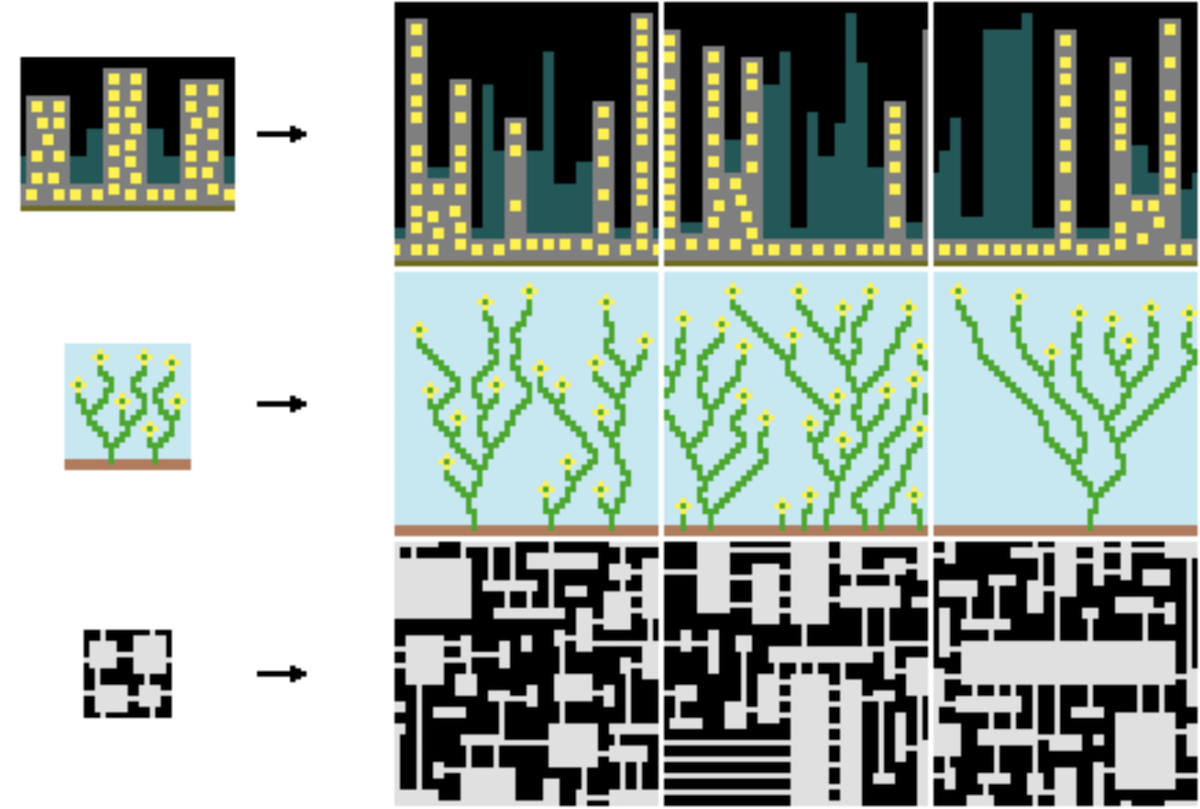
\includegraphics[scale=0.6]{obr/wfc-examples.png} % soubor + měřítko (scale)
  \caption{Příklad vzorů a výsledků \textit{WFC} \cite{waveClanek}} % popis obrázku
  \label{WFC_priklad} % definice odkazu na obrázek (pro \ref{})
\end{figure}

\subsection{GAN (Generative Adversarial Networks)}

\textit{Generativní adversariální sítě (GAN)} je metoda generování obsahu složená ze dvou komponent -- generátoru a diskriminátoru které "bojují" v procesu učení. Generátor vytváří realistické výstupy napodobující reálná data. Diskriminátor se pak snaží rozlišit zda jsou data reálná nebo vygenerovaná.

Princip metody \textit{GAN} právě spočívá v interakci mezi generátorem a diskriminátorem, díky které dochází k postupnému učení obou a tedy zlepšování kvality výsledných dat. Tento proces je řízen pomocí zpětné propagace, která umožňuje optimalizovat váhy v obou sítích. Toto vzájemné "soupeření" má za následek, že výsledná data systému \textit{GAN} vypadají realisticky i s menším množstvím vstupních reálných dat.

Mezi různé varianty \textit{GAN} patří například \textit{Deep Convolutional GAN (DCGAN}), který používá konvoluční vrstvy k lepšímu zachycení prostorových vzorců v datech. Tento přístup je například využit možné využít při generování výškových map, nicméně má některá omezení, jako jsou problémy s velikostí a škálovatelností výstupů. Dále existuje, \textit{Spatial GAN (SGAN)} jedná se o vylepšenou variantu \textit{DCGAN}, která eliminuje plně propojené vrstvy a místo nich používá konvoluční vrstvy s \textit{krokem}, což umožňuje lépe zachovávat prostorové vztahy a zlepšuje efektivitu generování. \cite{GANclanek}



\section{Porovnání metod}

Popsali jsme několik možných přístupů generování herních map. V této části porovnám popsané metody generování map a zvolím vhodnou metodu kterou implementuji v rámci tohoto výzkumného úkolu. 

Cílem je generovat herní mapu pro svět složený z políček nebo dlaždic pro strategickou hru, tedy výstup by měl připomínat přirozeně vypadající mapu světa. Tedy metody které vytvářejí nesouvislé nebo lineárně rozdělené výsledky nejsou vhodné (nebudu se snažit generovat města, pouze krajinu). 

Zároveň, jelikož pro každou hru bude generována nová unikátní mapa, by bylo vhodné aby generování probíhalo v rozumném čase, tedy metody s nízkou výpočetní náročností budou preferované.

Následující tabulka \ref{tabulka_metod} popisuje výhody a nevýhody jednotlivých metod generování.



\begin{sidewaystable}
\centering
\begin{tabular}{|l|l|l|}
\hline
\textbf{Metoda}                 & \textbf{Výhody}                                                                                                                     & \textbf{Nevýhody}                                                                                  \\ \hline
Space Partitioning              & \begin{tabular}[c]{@{}l@{}}Logická a hierarchická struktura\\ Snadné dosažení konzistentních výsledků\\ Vhodné pro vnitřní prostory\end{tabular}                                        & \begin{tabular}[c]{@{}l@{}}Výsledky můžou působit pravoúhle\\ Nevhodné pro organické mapy\end{tabular}                                      \\ \hline
Agent-Based generování          & \begin{tabular}[c]{@{}l@{}}Přirozené, nelineární výsledky\\ Velká variabilita výsledků\\ Snadné přizpůsobení chování agentů\end{tabular}                                                & \begin{tabular}[c]{@{}l@{}}Náročné ladění parametrů\\ Vysoká míra náhodnosti\\ Nepředvídatelné výsledky\end{tabular}                       \\ \hline
Grammar Algorithms              & \begin{tabular}[c]{@{}l@{}}Vysoká míra kontroly\\ Vhodné pro generování rozvržení úrovní\end{tabular}                                                                                   & \begin{tabular}[c]{@{}l@{}}Náročné na definování pravidel\\ Rychle narůstá složitost pravidel\\ Nevhodné pro přirozené terény\end{tabular} \\ \hline
Výškové mapy                    & \begin{tabular}[c]{@{}l@{}}Dobře reprezentují reálnou topografii\\ Plynulé přechody mezi výškovými úrovněmi\\ Snadná implementace \\ Snadná kombinace s dalšími technikami\end{tabular} & \begin{tabular}[c]{@{}l@{}}Náhodné generování vede k nereálným výsledkům\\ Nevhodné pro generování budov a interiérů\end{tabular}          \\ \hline
Fraktálové algoritmy            & \begin{tabular}[c]{@{}l@{}}Přirozeně vypadající krajina\\ Efektivní pro nekonečné terény\\ Relativně nenáročné na výkon\end{tabular}                                                   & \begin{tabular}[c]{@{}l@{}}Omezená kontrola\\ Výsledky mohou být homogenní\end{tabular}                                                    \\ \hline
Wave Function Collapse          & \begin{tabular}[c]{@{}l@{}}Konzistentní výsledky\\ Vhodné pro mapy s pravidelnými vzory\\ Snadné využití existujících vzorů\end{tabular}                                                                        & \begin{tabular}[c]{@{}l@{}}Výpočetně náročné\\ Složitý vstupní dataset\\ Může skončit ve stavu bez platného řešení\end{tabular}                                     \\ \hline
Generative Adversarial Networks & \begin{tabular}[c]{@{}l@{}}Realistické a variabilní výsledky\\ Adaptivní na různé typy prostředí\end{tabular}                                                                                                   & \begin{tabular}[c]{@{}l@{}}Velké množství trénovacích dat\\ Výpočetně náročné\\ Obtížně laditelné\end{tabular}                                                     \\ \hline
\end{tabular}
\caption{Porovnání metod generování prostředí}
\label{tabulka_metod}
\end{sidewaystable}

%_-------------------------------------------
%_-------------------------------------------
% GRAFICKY OPRAVIT; ZKONTROLOVAT GRAMATIKU
%_-------------------------------------------
%_-------------------------------------------
\newpage

Po porovnání metod generování map jsem se rozhodl využít \textit{metod výškových map}. Hlavním důvodem je, že tato metoda by měla být schopna generovat přirozeně vypadající krajinné útvary při poměrně nízké výpočetní náročnosti. Využití interpolace nebo gradientních metod umožní vytvářet plynulé přechody mezi různými tipy terénu, což povede k realisticky vypadajícímu světu.

Mou další volbou by byla metoda \textit{Wave Function Collapse (WFC)} případně \textit{Generative Adversarial Networks (GAN)}, jelikož tyto metody mají potenciál vést k ještě realističtějším a více rozmanitým výsledkům. \textit{WFC} by zajistilo více vzorů v prostředí, zatímco \textit{GAN} by umožnil generovat zcela nové mapy na základě trénovacích dat. Nicméně, obě tyto metody jsou výpočetně náročnější a vyžadují velké trénovací data, což je činní nevhodnými pro můj výzkumný úkol. Proto tyto metody ponechám jako případné možné rozšíření do diplomové práce.